\documentclass[12pt]{article}
\usepackage[nottoc]{tocbibind}
\usepackage[parfill]{parskip}
\usepackage{graphicx}
% \graphicspath{ {image/} }
\usepackage{geometry}
 \geometry{
 a4paper,
 total={170mm,257mm},
 left=20mm,
 top=20mm,
 }
\usepackage[
backend=biber,
style=ieee,
citestyle=numeric
]{biblatex}
\usepackage{listings}
\usepackage{color}

\definecolor{codegreen}{rgb}{0,0.6,0}
\definecolor{codegray}{rgb}{0.5,0.5,0.5}
\definecolor{codepurple}{rgb}{0.58,0,0.82}
\definecolor{backcolour}{rgb}{0.95,0.95,0.92}

\lstdefinestyle{mystyle}{
    backgroundcolor=\color{backcolour},
    commentstyle=\color{codegreen},
    keywordstyle=\color{magenta},
    numberstyle=\tiny\color{codegray},
    stringstyle=\color{codepurple},
    basicstyle=\footnotesize,
    breakatwhitespace=false,
    breaklines=true,
    captionpos=b,
    keepspaces=true,
    numbers=left,
    numbersep=5pt,
    showspaces=false,
    showstringspaces=false,
    showtabs=false,
    tabsize=2
}

\lstset{style=mystyle}
\usepackage[]{algorithm2e}
\usepackage{CJKutf8}
\usepackage{amsmath}
% \makeatletter
% \setlength{\@fptop}{0pt}
% \setlength{\@fpbot}{0pt plus 1fil}
% \makeatother
\addbibresource{biblio.bib}

\renewcommand{\baselinestretch}{1.5}
\renewcommand*\contentsname{TABLE OF CONTENTS}


\begin{document}

\begin{titlepage}
\begin{center}
        \vspace*{3cm}
        {\Huge A Question Answering System on SQuAD Dataset Using End-to-end Neural Network}\\

        \vspace*{3cm}
        {\Huge CS297 Report}\\

        \vspace{3 cm}
        Student: Bo Li\\
        Advisor: Dr. Chris Pollett\\
        Date: Dec 2017

 \end{center}
\clearpage
\end{titlepage}

\begin{titlepage}
\tableofcontents
\clearpage
\end{titlepage}



\section{Introduction}

Question Answering(QA) is about making a computer program that could answer questions in natural language automatically. QA techniques are widely used among search engines, personal assistant applications on smart phones, voice control systems and a lot more other applications.

In recent years, more end-to-end neural network architectures are built to do question answering tasks. In contrast, traditional solutions use syntactic and semantic analyses and hand made features. End-to-end neural network approach wins on giving more accurate result. However, traditional ways are more explainable. The neural network approach is used in this project.

Among rich and varied question answering data sets, the Stanford Question Answering Dataset(SQuAD) is used in this project. It includes questions asked by crowd workers on Wikipedia articles. The answer to each question is a segment of corresponding Wikipedia article\cite{rajpurkar2016squad}. In total, SQuAD contains 100,000+ question-answer pairs on 500+ articles\cite{rajpurkar2016squad}.


The goal of this project is to build a QA system on SQuAD using an existing end-to-end neural network architecture. If there is still time left after finishing the QA system, I will review related literatures and try to come up with an improved architecture.

This report is about the progress in CS297. Section \ref{sec:calculation}  corresponds to deliverable 1, which is a study on some very basic mathematics of neural network. Section \ref{sec:embdding} corresponds to deliverable 2, in which I did word embedding of Chinese classic poems. Please be noted, the project topic was changed in November 2017 and section \ref{sec:embdding} was not aimed at the current topic. Section \ref{sec:setup} and section \ref{sec:implementpaper} correspond to deliverable 3 and 4, which are about the current topic. Section \ref{sec:summary} includes my comment on my work in CS297 and my plan for next step.

\break

\section{Calculation of Back Propagation}\label{sec:calculation}

I calculated the back propagation on a dummy feed forward network example. I did this to convince myself this really works.


$$\hat{y}=softmax(z_2)$$
$$z_2=h\cdot W_2 + b_2$$
$$h=sigmoid(z_1)$$
$$z_1=x\cdot W_1+b_1$$

Define loss
$$J(W_1, b_1, W_2, b_2, x, y)$$
$$=cross\_entropy(y, \hat{y})$$
$$=-\frac{1}{D_y}\sum_{i=1}^{D_y}y_i \times \log{\hat{y_i}} $$

After using chain rules multiple times, I got

$$\frac{dJ}{dz_2}=\hat{y} - y$$
$$\frac{dJ}{db_2}=\frac{dJ}{dz_2}$$
$$\frac{dJ}{dh}=\frac{dJ}{dz_2}\cdot W_2^T$$
$$\frac{dJ}{dW_2}=h^T \cdot \frac{dJ}{dz_2}$$

\break

\section{Implementation of Word Embedding}\label{sec:embdding}

\begin{figure}[h]
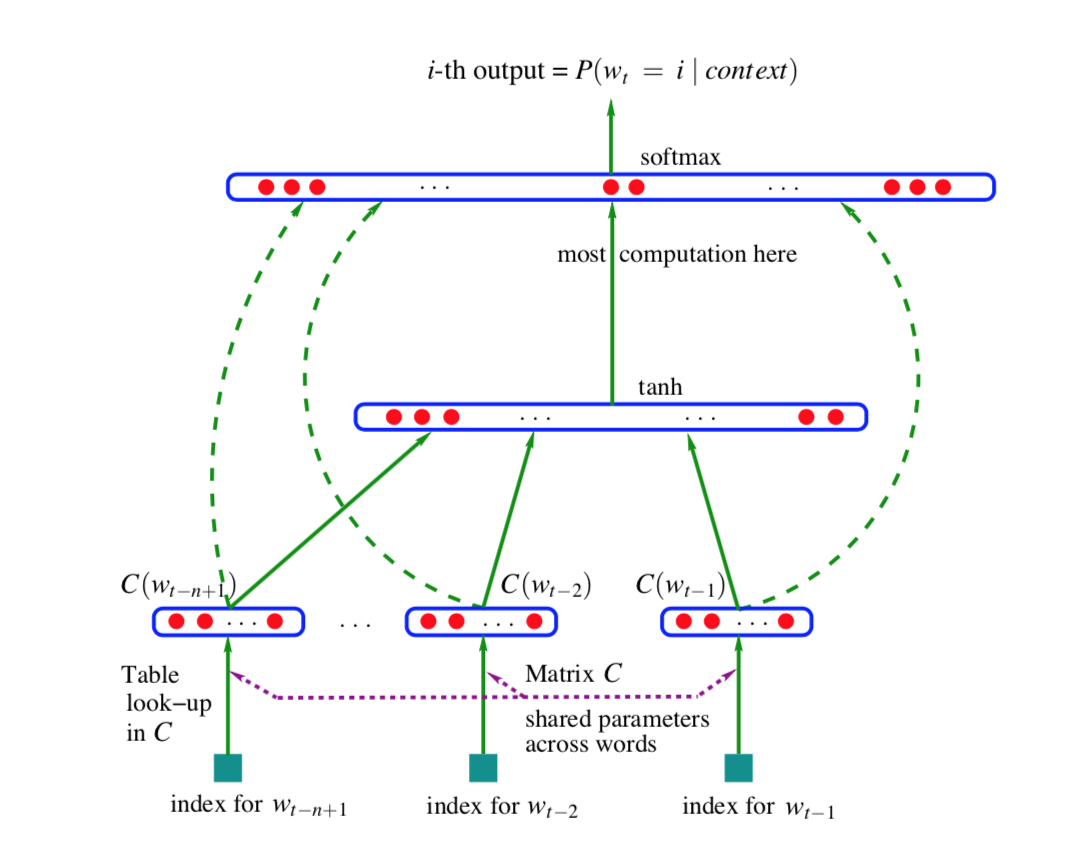
\includegraphics[width=15cm, height=10cm]{image/nplm_architecture.png}
\centering
\caption{Neural architecture: $f(i,w_{t-1},... ,w_{t-n+1}) =g(i,C(w_{t-1}),... ,C(w_{t-n+1}))$ where $g$ is the neural network and $C(i)$ is the $i$-th word feature vector\cite{bengio2003neural}}
\label{fig:nplm}
\end{figure}

Word embedding is a way to map each word to a feature vector in a continuous space. The dimension of the continuous space is much lower than the dimension of one-hot vector, which is comparable to the vocabulary size. Also, the distance between two word feature vectors could tell how likely the two corresponding words appear in same context.

Word embedding is originally introduced by  Bengio et al in \cite{bengio2003neural}. They propose a neural probabilistic language model(NPLM) which is illustrated in Fig.\ref{fig:nplm}. The trainning set is a sequence of words $w_1,...,w_T$ where $w_t \in V$ and V is the vocabulary. The purpose is to train a model $f$ such that $ \hat{P}(w_t | w_{t-1},...,w_{t-n+1}) = f(w_t, ..., w_{t-n+1})$. $f(w_t, ..., w_{t-n+1})$ is divided into two parts.
First, map each $w$ to a distributed feature vector by selecting the corresponding row in $C$.

$$x=(C(w_{t-1}),... ,C(w_{t-n+1}))$$

Second, $g$ maps $x$ to $f(w_t, ..., w_{t-n+1})$.


$$y=b+W\cdot x + U\cdot tanh(d + H\cdot x)$$
$$ f(w_t, ..., w_{t-n+1}) = \frac{e^{y_{w_t}}}{\sum_{i}^{}e^{y_i}}$$

The loss function to minimize is

$$L = -\frac{1}{T}\sum _{t}^{} \log{f(w_t, ..., w_{t-n+1})}$$


At the present time, an simplified architecture proposed by Mikolov et al in \cite{mikolov2013efficient} is widely used. The main difference between it and NPLM is Skip-gram removes tanh layer.

I implemented in Python both the NPLM model without Noise Contrastive Estimation (NCE) loss and skip-gram model with NCE loss. I use a collection of 284899 classic Chinese poems as the corpus.

Here are some information about the skip-gram together with negative sampling implementation. Training each epoch costs about 8 minutes. After about 5 epochs, the valid loss reaches the lowest. I selected 200 most common words and calculated cosine similarity between each two words pair to get 40000 word pair cosine similarity. Table \ref{table:similarity} lists top results among the 40000 results . According to my knowledge of Chinese classic poems, in most word pairs in Table \ref{table:similarity}, the two characters have high probability to appear in same context. As such, I think the model is implemented correctly.
\begin{CJK*}{UTF8}{gbsn}
\begin{table}[h!]
\centering
\begin{tabular}{c c c c }
作 后 0.999374 &
当 少 0.999315 &
同 好 0.999307 &
闻 好 0.999266 \\
同 少 0.999261 &
愁 闲 0.999212 &
好 少 0.999189 &
红 叶 0.999121 \\
复 少 0.999101 &
当 复 0.999071 &
故 少 0.999031 &
醉 闲 0.999025 \\
同 闻 0.999023 &
出 开 0.999002 &
空 入 0.999001 &
起 发 0.99899 \\
平 小 0.998955 &
亦 应 0.998954 &
雪 叶 0.998952 &
竹 叶 0.998946 \\
小 龙 0.998945 &
发 晚 0.998937 &
分 歌 0.99893 &
起 晚 0.998928 \\
寒 满 0.998914 &
过 向 0.998909 &
当 真 0.998894 &
入 阴 0.99889 \\
愁 后 0.998882 &
情 言 0.998881 &
尽 到 0.998878 &
当 故 0.998865 \\
到 起 0.998859 &
闻 少 0.998846 &
旧 少 0.998841 &
当 犹 0.998839 \\
开 阴 0.998839 &
复 物 0.998835 &
亦 还 0.998833 &
言 以 0.998825 \\

\end{tabular}
\caption{Most High Similarities Between 200 Most Common Words}
\label{table:similarity}
\end{table}
\end{CJK*}



\break

\section{Understanding Online Evaluation Environment and Setting Up Developing Environment}\label{sec:setup}


\subsection{Understanding Online Evaluation Environment}


Test data is not open to public. To evaluate a model, a prediction Python script should be submitted through Codelab.

As such, training and prediciton must be seprated. After training the mode, a tensorflow graph should be saved to disk. Then the prediction script should restore the tensorflow graph to make prediction on test data. This requires concise names and scopes for important nodes in the graph.


\subsection{Docker}

There are two main advantages to use Docker. First, the project goes more and more complex and software version dependency might cause problem. Second, I might need to use cloud GPU to train the model in the future and Docker helps on portability.

I followed the online installation instruction to install Docker on my mac book. Since setting up a Docker image is simply done by make a Docker file and typing a command in terminal, my developing speed is increase.

\break

\section{Implementating a Question Answering System Following
Paper \cite{wang2016machine}}\label{sec:implementpaper}

\subsection{Review on Paper \cite{wang2016machine}}\label{theoreticalModel}

Wang and Jiang \cite{wang2016machine} proposes an end-to-end neural network model on SQuAD dataset. While predicting, the inputs to the model are test data and pretrained word embeddings, the outputs are the predicted answers. While training, the inputs are train data and word embeddings, the outputs are losses to optimise. GloVe is used to do word embedding. The word embedding is not updated during training.

Model architecture includes three layers-the LSTM preprocessing layer, the match-LSTM layer and the Answer Pointer(Ans-Ptr) layer.

The LSTM preprossing layer encode each word sequence in passage and question to a sequence of hidden states using a standard one direction LSTM. The passage and question are processed separately.

$$H^p = \overrightarrow{LSTM}(P)$$
$$H^q = \overrightarrow{LSTM}(Q)$$

where

 $$P\in R^{d \times p}: passage$$
 $$Q\in R^{d \times q}: question$$
 $$H^p\in R^{l \times p}: encoded\ passage$$
 $$H^q\in R^{l \times q}: encoded\ question$$
 $$p: length \ of\ passage$$
 $$q: length\ of\ question$$
 $$l: dimension\ of\ LSTM\ hidden\ states$$
 $$d: dimension\ of\ word\ embedding$$

The match-LSTM layer uses the model in paper \cite{wang2015learning}. In this layer, a word-by-word attention mechanism and a LSTM are used together to encode hidden presentations of both passage and question to one sequence of hidden states that indicate the degree of matching between each token in the passage and each token in the question. To be specific,

$$\overrightarrow{G} = tahn(W^qH^q + (W^p{h_i}^p + W^r\overrightarrow{{h_{i-1}}^r} + b^p) \otimes e_q)$$
$$\overrightarrow{\alpha _i} = softmax(w^t\overrightarrow{G_i} + b \otimes e_q)$$


where

$$W^q, W^p, W^r\in R^{l \times l} $$
$$b_p, w\in R^{l}  $$
$$b \in R $$
$$\overrightarrow{{h_{i-1}}^r}\in R^{l}: one\ column\ of\ H_p  $$

and

\[ \overrightarrow{z_i} =
\begin{bmatrix}
{h_i}^p \\
H^q\overrightarrow{ {\alpha _i}}^T \\
\end{bmatrix}
\in R^{2l}
\]
$$\overrightarrow{{h_i}^r} = \overrightarrow{LSTM}(\overrightarrow{z_i}, \overrightarrow{{h_{i-1}}^r})$$

After iterating between getting attention vector $\overrightarrow{\alpha _i}$ and getting hidden state ${{h_{1}}^i}$ $p$ times, we get $[{{h_{1}}^r}, ..., {{h_{p}}^r}]$. Concatenate them to get

$$\overrightarrow{H_r} = [{{h_{1}}^r}, ..., {{h_{p}}^r}] \in R^{l \times p}$$.

To go over passage from both directions to get context information both before and after each word, go over $H_p$ from right to left to get $\overleftarrow{H_r}$. Then concatenate $\overrightarrow{H_r}$ and $\overleftarrow{H_r}$ to get

\[ H_r =
\begin{bmatrix}
\overrightarrow{H_r} \\
\overleftarrow{H_r} \\
\end{bmatrix}
\in R^{2l \times p}
\]
The Answer Pointer layer is motivated by the Pointer Net in paper \cite{vinyals2015pointer}. It has a similar structure with match-LSTM. However, instead of aiming at a sequence of hidden states, Ans-Ptr layer aims at the weight vector. Here I only explain the boundary model, which I will implement.

$$F_k = tahn(VH_r + (W^a{h_{k-1}}^a +  b^a) \otimes e_p)$$
$$\overrightarrow{\beta _k} = softmax(v^tF_k + c \otimes e_p)$$


where
$$V \in R^{l \times 2l}$$
$$W^a\in R^{l \times l} $$
$$b_a, v\in R^{l}  $$
$$c \in R $$
$$\overrightarrow{{h_{k-1}}^a}\in R^{l}: hidden\ state\ at\ positiom\ i\ of\ answer\ LSTM  $$

and answer LSTM is


$$\overrightarrow{{h_k}^a} = \overrightarrow{LSTM}(H^r\beta _k^T, h_{k-1}^a)$$

By iterating between the attention mechanisim and the answer LSTM two times, we could get $\beta _0$ and $\beta _1$. Let $a_s$ denote start index of the answer, and $a_e$ denote the end index, then we have

$$p(a|H^r) = p(a_s|H_r)p(a_r|H_r)=\beta _{0, a_s} \times \beta_{1, a_e}$$

where $$\beta_{k, j} = jth\ token\ of\ \beta _k$$.

To train the model, the loss function below is minimized.

$$J(\theta) = -\frac{1}{N}\sum_{i=1}^{N} \log{p(a^n|H^r)} $$


\subsection{Implementation Architecture}\label{sec:architectures}


\begin{figure}[h]
\includegraphics[width=16cm, height=16cm]{image/wangAndJiang.png}
\centering
\caption{Implementation Architecture of Paper \cite{wang2016machine}}
\label{fig:wangAndJiang}
\end{figure}

As indicated in Fig.\ref{fig:wangAndJiang}, the train pipeline, valid pipeline and evaluate pipeline are separated. This not only separates developing and deploying, but also make the large system easier to debug.

Take the train pipeline as example. The \texttt{preprocess.py} reads a json file, splits out passages, questions and answers, tokenizes them, and outputs each passage, question or data in token sequence. The \texttt{midprocess.py} reads token sequences and word embedding GloVe, vectorized token sequences to vector sequences, trims or pads the sequences, makes mask tensor, and outputs feed-ready data. The \texttt{train.py} takes feed-ready data and \texttt{model.py}, iterate through different number of epochs, learning rates, trainning optimizer and so on, and store trained models to disk.


Since Tensorflow graphs are shared in train, valid and evaluate steps, the feed data in the three steps must be consistent with the graphs. Since a graph is defined using pass\_max\_length, batch\_size, embed\_size, and  num\_units, which is called $l$ in theoretical model, train, valid and evaluate data are vectorized, padded, and divided to mini batches in same file \texttt{midprocess.py} using same pass\_max\_length, all data must be divided to same batch\_size. The num\_unit does not relate to shape of feed data.


To achieve batched training, paragraphs should be padded to same length, so does questions. As such, the model in implementation has some difference with the theoretical model explained in \ref{theoreticalModel}.

In preprocessing layer,
$$H^p = H^p \circ passage\_mask$$
$$H^q = H^q \circ question\_mask$$

In match-LSTM layer,
$$\overrightarrow{\alpha _i} = softmax( (w^t\overrightarrow{G_i} + b \otimes e_q) \circ question\_mask)$$


$$H_r = H_r \circ passage\_mask$$

In Ans-Ptr layer,
$$\overrightarrow{\beta _k} = softmax( (v^tF_k + c \otimes e_p) \circ passage\_mask)$$

\break

\section{Summary}\label{sec:summary}

I have made several milestones to myself in CS297. First, I have implemented Skip-gram model on Chinese classic poems data successfully. This is a milestone to me since I didn't know neural network and word embedding when I started this project. Second, I am able to understand paper \cite{wang2016machine}. This is a milestone to me since I experienced a long way to this including learning feed forward network, learning RNN, learning LSTM, and  learning attention mechanism. Third, I have designed a nice architecture and wrote some coding for implementing paper \cite{wang2016machine}.

The next step is to finish implementing paper \cite{wang2016machine} as soon as possible. And I will decide what to do next depending on the finish date.

\break



\printbibliography[heading=bibintoc,title={References}]


\end{document}
